\documentclass{article}
\usepackage[utf8]{inputenc}
\usepackage{amsmath}
\usepackage{amssymb}
\usepackage{color}

% For figures
\usepackage{graphicx,xcolor} % more modern
%\usepackage{epsfig} % less modern
\usepackage{subfigure} 

\newtheorem{definition}{Definition}

%\newcommand{\comment}[3]{}  % suppress comments
\newcommand{\comment}[3]{{\color{#1} {\bf #2 :} #3}}

\newcommand{\yoav}[1]{\comment{magenta}{Yoav}{#1}}
\newcommand{\piya}[1]{\comment{blue}{Piya}{#1}}
%\newcommand{\peter}[1]{\comment{purple}{Peter}{#1}}
\newcommand{\peter}[1]{\comment{pink}{Peter}{#1}}
\newcommand{\rayan}[1]{\comment{red}{Rayan}{#1}}
\newcommand{\alex}[1]{\comment{green}{Alex}{#1}}

%math symbols
\newcommand{\R}{\mathbb{R}}
\newcommand{\rad}{\mathcal{R}}
\newcommand{\sign}{\mathrm{sign}}


\title{HDR TRIPODS: From detection to reaction - computation in resource constrained sensor networks}
%\author{yfreund }
%\date{March 2019}

\begin{document}

\maketitle
%\yoav{We should define, in the introduction, some repeating terms, including compressed sensing and sketches. Maybe also more technical terms such as kernel, low rank matrices and low magnitude vectors/matrices.}\rayan{+ JL lemma}

\section{Summary}
Any agent, be it a human, an animal or a robot, has to react to it's environment to take advantage of opportunities and to avoid dangers. The transformation of events to reaction can be partitioned into three steps: {\bf(1)} {\bf physical events} are transformed by sensors into {\bf raw data}, {\bf (2)} Computation transforms the {\bf raw data} into {\bf knowledge} (a representation of the environment), and {\bf (3)} an {\bf action} is chosen based on the acquired {\bf knowledge}.

\rayan{I think we need to edit this a little. The first and second paragraphs feel disconnected from each other.}

The design of the sensors is dominated by considerations of sensitivity and resolution (temporal and spatial).  The goal is to detect the smallest, faintest and most transient signals,
by exploiting priors on the physical model of signal acquisition, and the geometry of signal representation. Computation is used to reduce raw data into an internal representation and then into actions. 

These days the leading architecture of reactive systems is wireless sensor networks. Sensor networks consist of large numbers of small independent units, each with sensors, computation and wireless communication. Such systems are constrained by power and communication bandwidth. 

One important consequence of these constraints is {\em pushing computation to the edge}. Instead of communicating the raw information from each sensor to a central computer, each sensor unit locally computes summaries, or sketches, which are shorter and therefore cheaper to communicate. This also reduces the computation load on the units that receive the information.

\section{Framework}
\newcommand{\state}{\theta}
\newcommand{\estate}{\hat{\theta}}
\newcommand{\Vstate}{\Theta}
\newcommand{\eVstate}{\hat{\Theta}}
\newcommand{\Sstate}{\psi}
\newcommand{\eSstate}{\hat{\psi}}
\newcommand{\VSstate}{\Psi}
\newcommand{\eVSstate}{\hat{\Psi}}
\newcommand{\env}{\mathbf{E}}
\newcommand{\transfer}{\mathbf{\Phi}}

\newcommand{\signal}{\mathbf{x}}
\newcommand{\Vsignal}{\mathbf{X}}
\newcommand{\dsignal}{\mathbf{y}}
\newcommand{\Vdsignal}{\mathbf{Y}}
\newcommand{\dtime}{t}
\newcommand{\ctime}{\tau}

\begin{figure}[t]
\centering
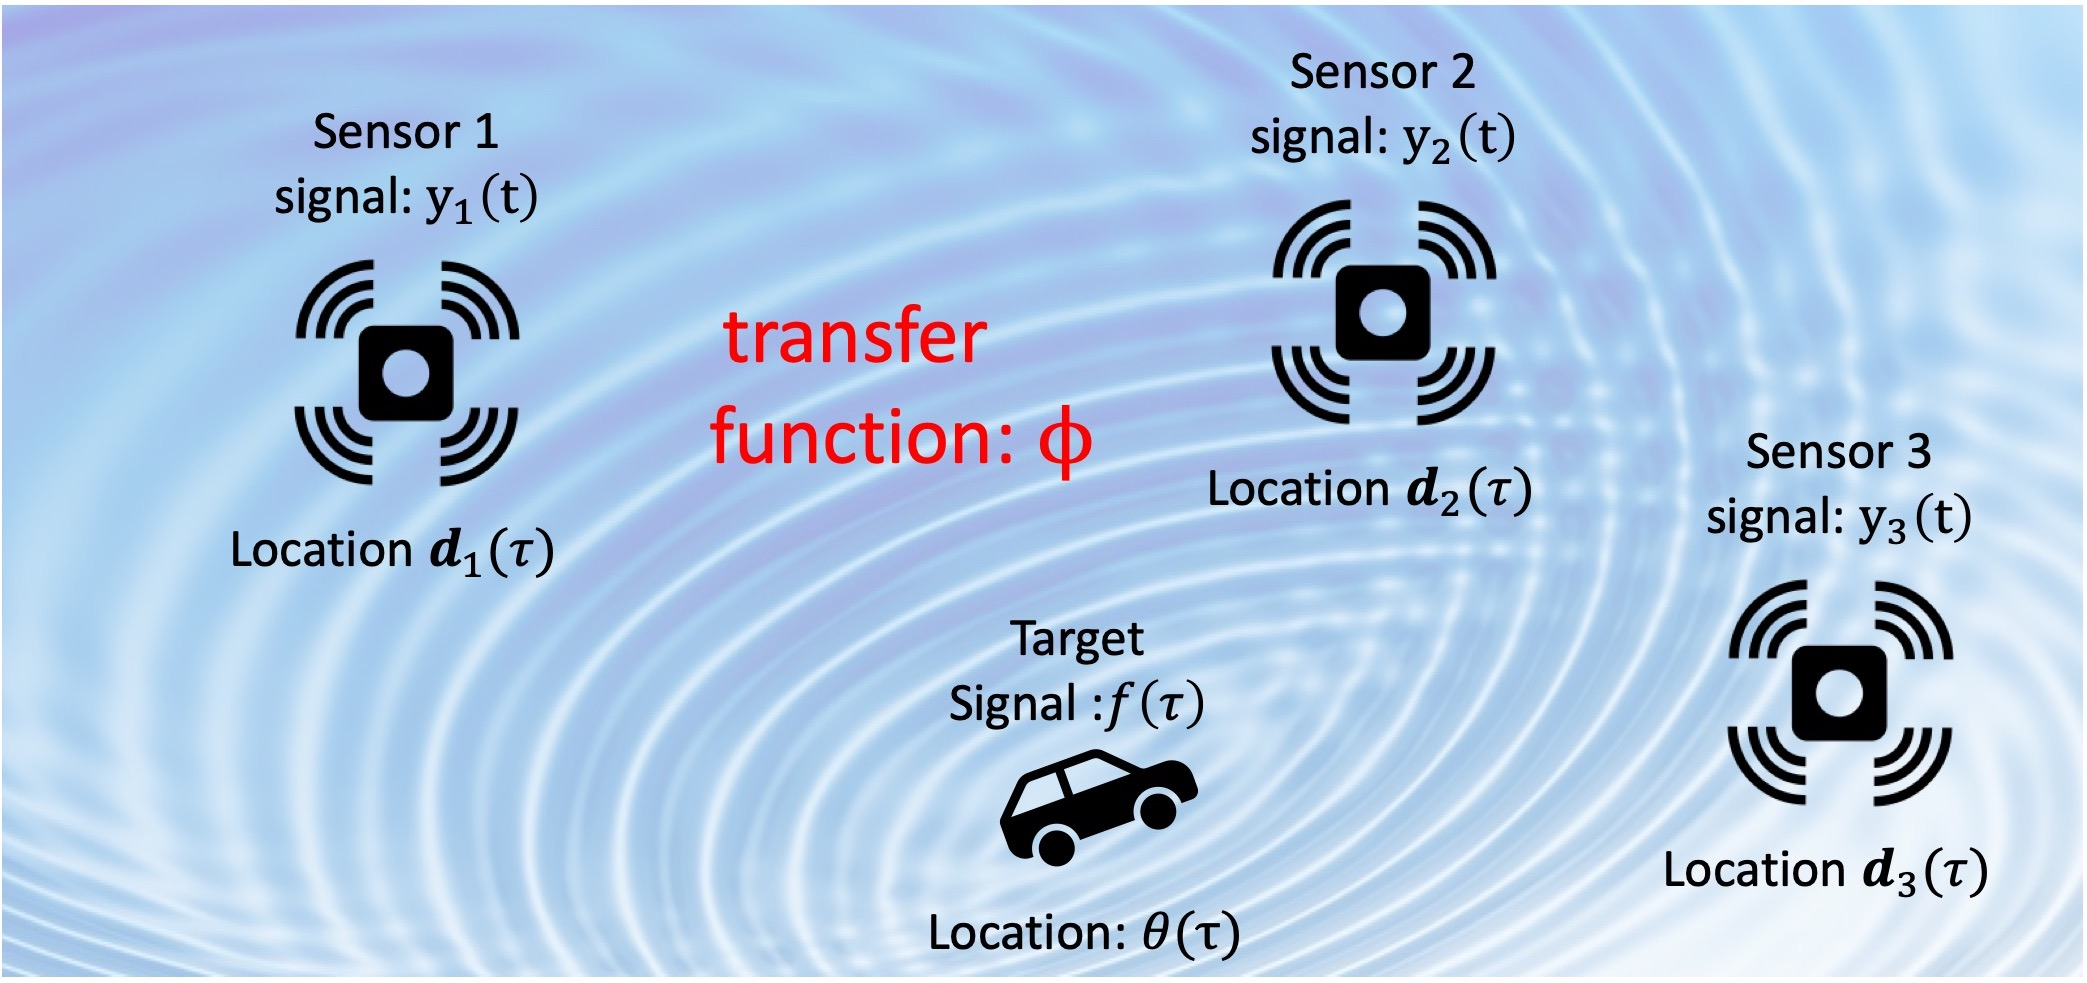
\includegraphics[width=0.9\columnwidth]{figs/Framework.jpg}
\caption{An example of a sensor network\label{fig:prototypicalSensorNetwork}. The goal of the network is to track a car. The location of the car as a function of time is $\theta(\ctime)$, and the goal of the network to produce $\estate(\ctime)$. The car emits a sound wave, which we denote by $x(\ctime)$. The sound wave travels through the physical environment and arrives at each sensor $i$, where it is digitized and made into a time sequence $y_i(\dtime)$. The transformation of the signal $x(\ctime)$ into $y_i(\dtime)$ is represented by a transfer function $\phi$. In this car tracking example 
$y_i(\dtime) = \phi(x(\ctime),\state(\ctime),\Sstate_i(\ctime))$\rayan{$\psi$ is not defined here}. We are seeking an inverse transformation that would map the measurements vector $y_1(\dtime),y_2(\dtime),y_3(\dtime)$ to an estimate of the car location $\estate(\dtime)$}
\end{figure}

This proposal combines several related lines of work. To facilitate the exposition, we start by introducing some terminology and notation that will be used throughout. {\bf Figure~\ref{fig:prototypicalSensorNetwork}} describes a simple sensor network that tracks a car using the sound waves the car is emitting.

We now expand this simple example into a more general framework.
We assume that the network consists of a $n$ sensors and $m$ 
targets. Sensor $i$'s state at time $\ctime$ is denoted $\Sstate_i(\ctime)$.  Similarly, the state of target $j$ at time $\ctime$ is denoted $\state_j(\ctime)$.
Here and in the rest of this section, we don't specify the spaces in which  $\Sstate_i$ or $\state_j$ are members. This allows for a general introduction, and more which will be made more specific in later sections. When appropriate, we will denote the combined state of all targets by $\Vstate(\ctime)$ and the combined state of all sensor by $\VSstate(\ctime)$. The third state component is the state of physical environment in which the targets and sensors reside. We denote the state of the environment by $\env(\ctime)$

The targets generate signals, which we call the {\em raw} signals. We denote the raw signal generated by target $i$ as $\signal_i(\ctime)$. We denote the collection of all $m$ signals by $\Vsignal(\ctime)$. On the receiving end, each sensor $i$ captures a digital signal $\dsignal_i$. These digital signals are the inputs to the computations we will discuss. As the signals arrive at physically separated sensors, the computation is inherently distributed. The main goal of this proposal is to develop algorithms that achieve desired tasks with minimal communication between the sensors.

\rayan{How are we deciding what variables are in bold and what variables are not? For example, why is $y_i(t)$ not bold in the caption, but $\mathbf{x}_i(\tau)$ in bold?}

The transfer function $\transfer$ defines the way by which the raw signals $\Vsignal$ are transformed into the digitized signals $\Vdsignal$. This function represents both the point transfer function of the physical environment,
the analog-to-digital transformation of the physical signal into a discrete time physical signal, and the noise that is added through this process. The transformation is defined by:\footnote{Note that the transfer function $\transfer$ operates on the whole sequences, not just on the sequence at a single time $\ctime$. That is because signal propagation takes time, so $\Vdsignal(\dtime)$ depends on $\Vsignal$ at multiple time points.}
\[
\Vdsignal = \transfer(\Vsignal,\Vstate,\VSstate,\env)
\]
Many of the problems we plan to tackle in this proposal are inverse
computation problems. We assume that some aspects of the physical
space are known, i.e. we know a subset of
$\Vsignal,\Vstate,\VSstate,\env$. Given the digitized signals
$\Vdsignal$, our task is to estimate the unknown parts of the physical
space. Reliable methods for computing such estimates exist. However,
they typically require high communication bandwidth. The goal of this
proposal is to find distributed estimation algorithms that achieve
good performance while using significantly less communication.

\subsubsection*{Some specific tasks}
We give a few specific examples of tasks. We will elaborate on some of these tasks below
\begin{enumerate}
    \item {\bf Target Localization:}
      Figure~\ref{fig:prototypicalSensorNetwork} depicts an archetypal
      target localization task. In this case the locations of the
      sensors $\VSstate$ and the state of the environment $\env$ are
      assumed to be fixed. A typical additional assumption, which is
      represented in the transfer function $\transfer$, is that
      strongest signal corresponds to the straight line of
      transmission between the target and the sensors. A common
      approach to target localization is to estimate the delay between
      the arrival of the signal at different sensors by using some
      type of cross correlation~\cite{}. This calculation is performed  
      It is well known that placing sensors far from each other provides the most accurate localization. However, achieving this accuracy with bounded communication between the sensors remains a challenge.
    \item {\bf Signal reconstruction} Voice based systems such as speakerphones, and voice activated computers, need to reconstruct the speech signal. Microphone arrays are sensor networks where the sensor is a microphone. Accurately reproducing the speech signal when there is more than one speaker is an open challenge. In this problem the location of the sensors is known, the goal is to reproduce the raw signal $\Vsignal$ where the environment $\env$ is unknown and the transfer function $\transfer$ is complex (reverberating environment).
    
    
    \item {\bf Optimizing sensor placement:} The accuracy of target localization depends on the location of the target and of the sensors. While the location of the target is not under our control, the location of the sensors is. Methods for optimizing the locations of the sensors will be described in Section~{sec:sensor-placement.}
    
    \item{\bf Mapping the environment} Sometime the goal of the system is to estimate the environment $\env$. One example is to use Radar, Sonar or Lidar to create a 2D or 3D representation of the environment for a smart car. Another example, coming from seismology is to use controlled vibration sources and many acceleration sensors to map the subterranean earth. In these settings the locations of the sensors $\VSstate$ and the targets $\Vstate$ (called transmitters in this context) is fixed and known, as is the raw (transmitted) signal $\Vsignal$. The goal is to deduce $\env$ from the collected signal $\Vdsignal$. (Peter, does this make sense to you, can you use this formulation in your sections about tomography and dictionaries?)
    
    \item {\bf Monitoring} In many situations the goal of the sensor network is to track the environment, identify trends and detect anomalies. Motivating examples include: Security systems, systems for monitoring patients or the elderly, highway monitoring and factory floor monitoring. Many of these environments are too complex to estimate a fully detailed representation. Instead, we suggest building a statistical model which implicitly captures the major degrees of freedom of the environment and the way they relate to major variables such as time of day and day of week.  The challenge here is to learn such a model in an unsupervised or weakly supervised way, without heavy use of computational or communication resources. Here, we will propose, and rigorously analyze techniques based on Kernel methods combined with sketching and low dimensional binary embedding techniques. The combination of these tools will simultaneously facilitate performing various desired statistical tasks, while minimizing storage, communication, and computational costs. 
    
\end{enumerate}

\subsection{Target Localization using minimal number of sensors}
\yoav{Piya, can you use the notation I defined in the framework
  section? Also I would like to merge this  subsection and the
  following one, which describes sensing geometry and the goal of
  minimizing the number of sensors.}
A sensor network consisting of $M$ sensing units aims to capture information of interest (often described in terms of parameters) regarding the physical environment by acquiring measurements in space (dictated by sensor locations) and in time (dictated by the sampling technique employed at each sensor). In many applications (especially those concerning high-resolution/super-resolution imaging), the goal is to detect certain parameters $\theta_i\in\mathbb{C}^P, i=1,\ldots,K$ from $K$ targets of interest in the environment by acquiring signals emitted by them. 

\yoav{This describes a more general framework, using $\mathbb{C}^P$ (does that mean each coordinate is complex?). What is gained from this generality? maybe drop the general notation? Also how does high resolution/super-resolution fit here? If you have worked on such problem, I suggest you devote a paragraph and cite, rather than just mentioning in passing.} 

As an example, consider a network consisting of active radar units (for example, those mounted on autonomous vehicles) attempting to create a map of the environment. In this case, $K$ can denote the total number of pedestrians, bicyclist's and other cars and $\theta_i\in\mathbb{R}^3$ for the $i$th target will consist of its location $\mathbf{x}_i=[x_i,y_i]^T$ and velocity $(v_i)$ parameters, i.e.
\begin{equation} \theta_i = [ x_i, y_i, vx_i ,vy_i]^T, \quad 1\leq i\leq K  
\end{equation} 
\yoav{Shouldn't $K$ be estimated?}
%\rayan{It could also be 3 dimensional :), as can position}
Mathematically the space-time measurements collected at the $m$th sensing element can be described as \begin{equation} 
y_m (t) = \sum_{i=1}^{K} \phi (\mathbf{d}_m,\theta_i,t) + w_m(t), \quad 1\leq m\leq M
\end{equation}
where $w_m(t)$ is the additive noise. Here $\mathbf{d}_m\in \mathbb{R}^3$ denotes the location of the $m$th sensor and the function $\phi(.)$ characterizes the measurement model (often referred to as the point-spread function in the context of imaging) that depends on the physical laws governing wave propagation, and properties of the medium. Depending on the application and model assumptions, the function $\phi(.)$ can be linear, non-linear, and potentially, even non-convex. However, it can be {\em partially designed} by choice of senor locations $\mathbf{d}_m$. This will be a key enabler towards obtaining compressed sketches of measurements (or reducing the number of sensing units) while preserving the ability to reliably infer the parameter $\theta_i, 1\leq i\leq K$.\\

The basic model assumes targets as point sources, but in many situations, they are distributed. \piya{Perhaps Peter can help characterize this model, since SONAR deals with such targets}. 

The main objective is to obtain estimates $\hat\theta_i, 1\leq i\leq K$ of the parameters of interest ($\theta_i$) using {\em minimal number of measurements/minimizing the number of sensing elements}. These estimates essentially are some appropriate functions of the spatio-temporal measurements $Y_T = \{y_m(t),  1\leq m\leq M, 1\leq t\leq T \}$, i.e., \begin{equation}
\hat{\theta_i}(T) = g_i (Y_T) 
\end{equation} 
%\subsection*{Central Objective and Role of Sensing Geometry (Piya)}
In many scenarios, the parameters of interest can be reliably inferred from the {\em correlation of the measurements}. In other words, the correlation of the measurements act as a sufficient statistic for the parameters to be inferred. Depending on the application, the correlation matrix can be spatial (when the source signals are stationary), or spatio-temporal (when the temporal dynamics need to be tracked, such as for change-point detection). In these cases, we can effectively summarize the large amount of raw sensor measurements by only retaining and communicating their correlation. 
\yoav{The way I was thinking about it, each sensor has only one signal. In a one scenario, the quantity of interest is the "time delay of arrival" or the time shift of one signal relative to another that would maximize the correlation. Is there anything known about computing this time delay without communicating the whole time series?}

\noindent{\bf Spatial Correlation and Localization:} Suppose we compute the spatial correlation between $y_m(t)$ and $y_n(t)$  by averaging over $T$ time samples (the signals are assumed to be stationary over this interval) \footnote{Reasonable to do so when the source signals are stationary and emit independent signals. This is the common practice in source localization using antenna arrays. We can also use more sophisticated regularized estimation of correlation.}
\begin{equation}
r_{m,n} (T) = \frac{1}{T}\sum_{t=1}^{T} y_m (t) y^*_n (t) 
\end{equation} 
We can summarize the self and cross correlation between $M$ time-series measurements (collected at $M$ sensors) using these $M^2$ correlation values (collected in the form of a correlation matrix $R_T$). Owing to the geometry of the measurements, these correlation values directly depend on the sensor locations $\mathbf{d}_m$  (via the mapping $\phi(.)$). Hence, it is natural to ask 
\begin{enumerate}
\item Can we exploit the geometry of the measurement model to further compress the  correlation matrix $R_T$? What is the role of sensor geometry in this case? We should still be able reliably infer $\theta_i, i=1,2,\ldots, K$ from such a compressed sketch.
\item How large should $M$ be (in comparison to $K$) ?
\end{enumerate}

\section{Correlation-Aware Sensing (Piya)}
\yoav{How is this problem different from the problem of finding the
  best placement for the sensors in order to maximize the accuracy of
  localization, ignoring communication bendwidth?}

With the aim of obtaining a compressive sketch of the correlation matrix (also termed as compressive covariance sensing), we will optimize the design of sensor array (i.e. choice of $\mathbf{d}_m, 1\leq m\leq M$) by understanding how the array geometry controls the algebraic structure of $R_T$. One of the main objectives will be to understand how much communication is needed (and between which subset of sensors) to achieve a certain level of accuracy. To illustrate this, we briefly discuss Co-PI Pal's recent work in structured sampler design (e.g., nested, coprime and generalized nested samplers) which utilize the idea of difference sets.

\begin{itemize}
\item {\bf Difference set-inspired Designs:} I will review some results in the context of array processing and DOA estimation...(to be filled in).
\item {\bf Proposed Research:} Motivated by these results, our goal will be to develop a rigorous framework for further developing the key idea of correlation-aware sensing to a distributed scenario and make it applicable for imaging problems beyond point target localization.
\begin{enumerate}
\item {\bf Distributed Sensing:} The idea of difference set inspired sampler design can be actually generalized beyond that of antenna arrays, to acquire {\em compressive sketches} of the correlation between signals acquired between pairs of sensors. In general, given $N$ sensors, it is natural to think that one needs to compute the correlation between all $N\choose 2$ time series (from all possible sensor-pairs) to construct the overall $N\times N$ correlation matrix $R_T$. However, using the idea of difference-set sampling, one can only compute  cross-correlation values between a much smaller subset of size $\Theta(\sqrt{N})$ of {\em suitably selected sensor-pairs} and recreate the entire $N\times N$ correlation matrix $R_T$. In the context of distributed sensing, this automatically means that only these sensors need to communicate and exchange information.

{\em Exploiting Distance-based Redundancies:} The key idea behind achieving such reduction is to exploit the redundancies present in the correlation values that naturally result from the physical spatial signal model. A widely used example of such a redundancy is that the correlation $r_{m,n} = E\Big(y_m(t)y^*_n(t)\Big)$ between $m$th and $n$th sensors is of the following form \begin{equation} r_{m,n} \approx f(\mathbf{d}_m - \mathbf{d_n}) \label{eqn:CorrRed}\end{equation}
In other words, the correlation is spatially only a function of the {\em inter-sensor distance}, and this is a direct consequence of the functional form of $\phi(.)$ \piya{Can give specific examples if needed}. This is also referred to as spatial stationarity and it is (exactly or approximately) true for many applications as narrowband and wideband radar \footnote{In the latter case, this holds at individual frequency bands after splitting the wideband signal into narrow frequency bins using a filter bank}, super-resolution optical imaging \cite{}, mmWave wireless channels \cite{} and so forth. Hence, depending on the inter-sensor distances, many of these $N\choose 2$ correlation values are actually repeated/redundant. Based on this observation, we propose to use a new sketching technique developed by co-PI Pal, called {\bf Generalized Nested Sampling (GNS) to reduce the amount of inter-sensor communication}. Suppose the sensors are located on a uniform grid. In one dimension, (\ref{eqn:CorrRed}) implies that the correlation matrix $R_T$ has Toeplitz structure and GNS provides an optimal way to select sensors to sketch such a matrix. 
\begin{definition}\piya{Definition of GNS goes here..}
\end{definition}
Hence, GNS dictates how to select a subset $\mathcal{S}_{\text{GNS}}$ of $M =  = \Theta(\sqrt{N})$ sensors out of $N$ available sensors. Let $R_{\mathcal{S}} \in \mathbb{C}^{M\times M}$ be the correlation matrix computed by aggregating the signals from these sensors. Then GNS ensures that $R_{\mathcal{S}}$ is a {\em lossless} sketch of the high-dimensional correlation matrix $R_T$. \piya{To Add (i) Finite sample performance guarantees (ii) two and three-dimensional extension (iii) low-rank extension and (iv) Time-varying model.}


%Will focus on what subsets of sensors in a distributed setting should communicate to be able to reconstruct the source scene. Can think of a subset of spatially close sensors to fully communicate with each other (assuming cost of communication proportional to proximity/distance), and then transmit the sketch / coarse parameter estimates (or their binarized measurement) to the sensors further away. Can lead to interesting hierarchical configurations for distributed sensors, dictated by $\phi(.)$. {\color{red} [To Add more Details..]}.
%\yoav{I think this is a very interesting question. Especially when the best subset depends on the location of the source.}\rayan{agree!}
\item {\em Beyond Point Target Localization: Using Priors and Sparsity} In many applications such as camera networks, the quantities of interest are not the low-level measurements acquired at the CCD sensors, but the processed images $I_t$. In such cases, we need to obtain a compressive sketch of the image $A (I_t)$ via the sketching operator $A (.)$ using low dimensional representation (over unions of subspaces or manifolds). In addition to conventional sparsity and low-rank priors, one can also utilize (partial) knowledge of the prior distribution of the images $I_t\sim~\mathcal{D}$. Utilizing these priors can lead to more effective compression for a given level of sparsity. {\color{red} [To be written..]}  
\end{enumerate}
\piya{These tasks can be further integrated with the binary embedding based sketching ideas proposed by Rayan and Alex.}
\rayan{Agree!}
\end{itemize}

\section{Localization of weak sources (Peter)}

\yoav{Can the description of SCM be folded into Piya's introduction?}

The focus here is detecting weak sources within a sensor network without a fusion center. To observe weak sources, as much information as possible should be used. Thus, at first there is no attempt to reduce the information in the data by sketching or special sensor arrangements. The network could consist of sensors with know location, partially unknown or unknown positions.

The propagation path from a given source location would here represent multiple propagation paths in a non-uniform media. The frequency domain transfer function from a source location to $N$ receivers ${\bf a}$. Assuming $K$ uncorrelated sources of complex amplitude ${\bf s}$ at spatial location ${\bf x}_k$, the received signal ${\bf y}\in {\cal R}^N$ on $N$ receivers is 
\begin{equation}
{\bf y}={\bf A}{\bf s}+{\bf n},
\end{equation}
where ${\bf A}=[{\bf a}_1, \ldots {\bf a}_K ]$  and $\bf n$ is uncorrelated noise. 
The sources might be located in the near field and  composed of many propagation paths. Examples of many propagation paths from a single source could be waves from  
1) a source in a house propagating though the air and though the wall.
2) a cell phone signal with a direct path, a reflected path or refracted path.
3) a car radiating noise though the air and though the ground.
Further, the sensors are not placed in a regular order, but where practical and maybe with unknown location. Thus the elements in ${\bf a}_k$ are unknown.

\yoav{What is the relationship between $a_k$ and $x_k$?}

To make observations of weak sources we observe $L$ snapshots  assuming  stationarity ${\bf Y}=[{\bf y}_1 \ldots {\bf y}_L]$.
We can here form the sample covariance matrix (SCM)
\begin{equation}
{\bf S} ={\bf Y}{\bf Y}^H/L
\end{equation}
and form the the normalized SCM $\hat{\bf S}$ or coherence with elements
\begin{equation}
{ S}_{ji} =\frac{{ S}_{ji}}{\sqrt{ { S}_{ii}{ S}_{jj}}}
\end{equation}

\yoav{I am confused about the definition of coherence, should it not be the maximum correlation when one signal to be shifted relative to the other?}

Forming the ensemble mean over multiple snapshots give the cross spectral density matrix${\bf C}\in {\cal R}^N\times N$
\begin{equation}
{\bf C}={\cal E}[{\bf y} {\bf y}^H]= {\bf A}{\bf s}{\bf s}^H{\bf A}^H+{\bf N},
\end{equation}

The array signal processing literature is ample with processing of this type, especially with the structure of the $\bf A$ matrix partially known. In this work we will focus on pushing the computations to the sensor nodes and thus only observing part of SCM.

\subsection{Graph signal processing approach without a fusion center}
\yoav{I think this section can be combined with Piya's
  sections. Choosing which pairs should communicate is clearly related
  to their geometric layout.}

Here the processing is done locally at each node. A graph signal processing approach was used in Ref \cite{riahi2017} for a 5000 element seismic array by processing the whole normalized SCM at once, i.e., using a fusion center. 
When the coherence $\hat{\bf S}$ is above a certain threshold at  element $ij$ it is likely that a signal is observed and has propagated between nodes $i$ and $j$, essentially forming an edge between nodes  $i$ and $j$ in a graph. When a sufficient set of connected edges are detected in a region of the network a source is likely in that region. Part of the extracted SCM can then be used localize the source more precisely.

To extract very weak signals with a well estimated and robust SCM is needed. Thus we  pass the full time series between local nodes $i$ and $j$, not the whole array and develop robust signal processing methods\cite{zoubir2018}. This will represent a lot of communication demand and thus we will only pass signal between neighboring stations. Once a graph edge is formed it could either be communicated further to a wider set of nodes.

Robust signal processing methods\cite{zoubir2018} would entail making the processing insensitive to outliers. Qualitative robustness can be investigated via the influence function. A qualitatively robust estimator is characterized by an IF that is continuous and bounded. Continuity implies that small changes in the observed sample cause only small changes in the estimate. The boundedness implies that a small amount of contamination cannot lead to an unbounded error the estimate.

\subsection{Tomography}
\yoav{I believe you are talking here about tomography, or reconstructing the environment. Can you write a paragraph of introduction, what is the problem? What is the desired solution?}
Sparse modeling assumes that signals can be reconstructed using a few (sparse) vectors, called atoms, from a potentially large set of atoms, called a dictionary. Recent ocean acoustics works utilizing sparse modeling is beamforming\cite{Xenaki2014}, matched field processing \cite{Gemba2017}, and geoacoustic inversion \cite{gerstoft2018}. One challenge in sparse modeling is finding the best dictionary for sparsely representing specific signals. Such dictionaries can be composed of wavelets, or the discrete cosine transform (DCT). These predefined dictionaries perform well for many signals. However, using a form of unsupervised machine learning, called dictionary learning, optimal dictionaries can be learned directly from specific data\cite{mallat1999}. It has been shown that learned dictionaries outperform generic dictionaries when sufficient signal examples are available. Machine learning, and specifically dictionary learning, have recently obtained compelling results in ocean acoustics cite{Bianco2017} and seismology\cite{kong2018}. 
\rayan{I might be able to throw in some text about learning fast dictionaries, i.e., dictionaries learned from the data, but that also admit fast transforms like FFTs.}
\yoav{The simplest type of Dictionary learning is learning a codebook for Vector Quantization. Dictionaries are different than VQ if they combine (add) multiple vectors to represent a singe location in the signal. Is there a chance that VQ methods might work?}


\yoav{I don't understand the following three paragraphs, can you give some technical details? Formulas?}
In current work, we have developed a machine learning-based travel time tomography method called locally sparse travel time tomography (LST)\cite{bianco2018}. In LST, small scale local features contained in small rectangular groups of pixels, called patches, in an overall slowness (inverse  speed) map are constrained using a sparse model. Further, the sparsifying dictionary is adapted to the specific slowness data using dictionary learning. Larger scale, or global features spanning the  map, are constrained with least-squares regularization. Unlike conventional tomography, in which model features are forced to be exclusively smooth or discontinuous, the LST approach permits smooth and discontinuous local features via dictionary learning. 


Whereas many machine learning techniques in geoscience\cite{kong2018}, are reliant on large amounts of training data, LST requires none. In LST we adopt the adaptive dictionary learning paradigm from image denoising \cite{elad2010} and medical imaging\cite{ravishankar2011}, in which dictionaries are learned directly from patches of the corrupted image. In LST, slowness dictionaries are learned from patches of a least squares regularized inversion, and are then used to reconstruct a sparsity-constrained slowness image. Assuming sufficiently dense ray sampling, the dictionary is initially unknown and is learned in parallel with the inversion. LST obtains high resolution by assuming that small patches of discrete slowness maps are repetitions of few elemental patterns from a dictionary of patterns. These patterns, which are described by the atoms in the dictionaries, are extracted from the data by dictionary learning. The increase in performance for synthetic slownesses relative to competing methods, are demonstrated for  ambient noise tomography\cite{bianco2018}. 

Assuming that the travel paths between sensors has been estimated\cite{sabra2005,gerstoft2006} We here propose the future development of machine learning-based tomography methods in ocean acoustics. Such methods will help to more fully-exploit both existing hydrophone and environmental data, as well as very dense sampling from future arrays with many sensors. Such large scale, mobile, and deformable arrays, will use ambient noise processing \cite{sabra2005}, to obtain very dense and rich data sets. We propose for future work to: (1) further develop a dictionary learning-based travel time tomography \cite{bianco2018}, accounting for uncertainty in the measurements and physics; (2) formulate the dictionary learning-based approach as CNN via CSC; and (3) apply this CSC tomography framework to  data assimilation, to obtain higher-resolution estimates of water column parameters over conventional methods. We further propose to develop  (5) acoustic event detection methods that leverage recent advances in machine learning.

\section{Fast binary embeddings... (Saab, Cloninger,...)}
\yoav{Rayan and Alex, please link your sections to one or more of the
  specific tasks above. Feel free to add other tasks, but these should
  be specific real world applications, not just mathematical frameworks.}
\rayan{{\bf Hi All: Please don't edit this section until after our meeting. Alex and Rayan are working on this. Comments welcome of course.}}

Consider an application where a network of sensors' goal is to detect whether a major change in the status of the system being observed has occurred. In such a setting, each sensor may collect, in an ongoing way, large amounts of data. However, communicating all this data across all the sensors to perform this statistical task may be prohibitively expensive and tremendously wasteful. Similarly, consider the (e.g., anomaly detection) setting where one may wish to determine whether data being collected at two sensors, or at two sets of sensors is similar (e.g., drawn from the same distribution), without communicating all the data across sensors. One way to alleviate the large communication costs associated with such problems is for each sensor to maintain only a binarized (or low bit-depth) sketch that is sufficient to perform the required statistical task (\cite{Gribonval, Jacques}). It is a main goal of this section to develop both algorithmic tools and rigorous theoretical analysis for this framework. 

%\rayan{working on this}
%Indeed, distributed systems often have severe bandwidth and energy constraints that necessitate only sketching (i.e., keeping a parsimonious representation) the data being sensed. Further, to minimize the computational and storage costs associated with such sketches, one may revert to 
We will rely on extremely
coarse, e.g., binary, quantization of the data-sketches. In addition to minimizing storage and computation costs (see e.g., \cite{fang2014sparse,boufounos20081}) these methods have the added benefit of being appealing in hardware implementation particularly if they are computationally inexpensive and consequently promote speed in hardware devices (\cite{jacques2013robust,le2005analog}). % (e.g, \cite{fang2014sparse,boufounos20081}). Additionally, simple binary representations of data can be also quite appealing in hardware implementations, particularly if they are computationally inexpensive and consequently promote speed in hardware devices (\cite{jacques2013robust,le2005analog}). On the other hand, a major concern in using very coarsely sketched data is possible loss of accuracy when performing various tasks of interest, ranging from signal reconstruction to clustering and statistical hypothesis testing, among others.
\subsection{Background and Prior Work}Indeed a growing body of work, which co-PI Saab has contributed significantly to (e.g., \cite{SaabIEEEIT,knudson2016one,saab2018quantization,LybrandSaab2018,iwen2019new}), has focused on signal reconstruction from coarsely quantized compressive measurements. One important theme that emerges from this line of work  is that if one collects more coarsely quantized measurements than a critical minimal number, and uses sophisticated quantization schemes, then the extra measurements can be efficiently used in quantization-aware algorithms to rapidly drive the reconstruction error down.

Co-PI Saab has recently  extended this observation  beyond signal reconstruction, to the context of (Euclidean) distance-preserving binary embeddings \cite{huynh2018fast}. To be precise, we now briefly describe this contribution as it is pertinent to our ensuing discussion. In \cite{huynh2018fast}  $A: \R^n \to \R^m$ is a \emph{random} Johnson-Lindenstrauss (i.e., distance preserving) map and  $\mathcal{T}\subset \R^n$ is a set of finite or infinite cardinality. Moreover, $Q:\R^m \to \{\pm 1\}^m$ is a noise-shaping quantizer (e.g., a $\Sigma\Delta$ \cite{stuff} or $\beta$ \cite{stuff} quantizer). In their most commonly used form, noise-shaping quantizers act sequentially on the measurements, say $y_i$. For example, the simplest noise-shaping quantization scheme, the so-called greedy $1$st order $\Sigma\Delta$ scheme, is given, for $i=1,...,m$, by 
\begin{align}
    q_i &= \sign(y_i+u_{i-1})\\
    u_i &= u_{i-1} + y_i -q_i,
\end{align}
where the state-variable sequence $u_i$ is initialized via, e.g., $u_0=0$. In matrix-vector notation, this yields the relationship \begin{equation}y=Du+q\label{eq:SD_state}\end{equation}  between the measurement vector, the state variables, and the resulting quantization, with $D$ being the $m\times m$ first-order difference matrix. Crucially both for the analysis and for practical implementation, this scheme is \emph{stable}, that is, \begin{equation}\|y\|_\infty \leq c_1 \implies \|u\|_\infty \leq c_2,\label{eq:stability}\end{equation}
for dimension independent constants $c_1,c_2$.

\yoav{How does one create an estimate of $y_i$ from $q_i$?}\rayan{see the blue text}{\color{blue}

For example, in the context of compressed sensing \cite{}, where the signals $x$ are sparse and the measurements are of the form $y = Ax$, one may recover an estimate $\hat{x}$ of $x$ from $q$ by solving an optimization problem  that encourages, say, sparsity, with the constraint that $\|D^{-1}(A\hat{x}-q)\|_\infty \leq c_2$. The constraint is critical; it ensures that the solution $\hat{x}$ respects the quantizer by satisfying \eqref{eq:SD_state}  and \eqref{eq:stability}}. More generally, other \emph{stable} noise-shaping quantizers act sequentially on the measurements $y_i$, %via carefully chosen functions $\rho,$
%\begin{align}
%q_i = \sign(\rho(y_i, u_i,u_{i-1},...,u_{i-r}))
%u_i = 
%\end{align}
%for carefully 
and yield relations of the form 
$$ y=Hu + q,$$ where $H$ is a lower-triangular matrix associated with the scheme. Quantizers of interest to us include
stable $r$th-order (with $r\geq 1$) $\Sigma\Delta$ schemes  \cite{}, with the relationship $y=D^r u+q$, and distributed-$\beta$ encoding schemes \cite{} where $H$ is a block diagonal matrix constituted of identical lower-triangular blocks, say $G$, given by $G_{i,i}=1, G_{i+1,i}=-\beta$, and $G_{i,j}=0$ otherwise.

With these quantization schemes playing a prominent role, in  \cite{huynh2018fast} co-PI Saab  constructed approximately isometric (i.e., distance preserving) embeddings between the metric space  $(\mathcal{T}, \|\cdot\|_2)$ and the binary  cube $\{-1,+1\}^m$ endowed with the pseudometric
$$d_{{V}}(\tilde{q},q) := \| {V}(\tilde{q} -{q}) \|_2$$
where $V$ is a carefully constructed matrix.
For a  matrix $A\in\R^{m\times n}$, and a noise-shaping quantizer $Q$, as above, the algorithm for computing these embeddings is simply given by \begin{align}
g: \mathcal{T} &\to \{\pm 1\}^m\nonumber\\
x &\mapsto q=Q(Ax).\nonumber
\end{align}
%\rayan{Perhaps we need a section where we introduce background material like the  Johnson-Lindenstrauss lemma?}

In particular, when $A$ is a fast Johnson-Lindenstrauss matrix (e.g., \cite{}), the constructed embeddings support fast computation, and despite their highly quantized non-linear nature, they perform as well as linear Johnson-Lindenstrauss methods up to an additive error that decays exponentially (for $\beta$ quantizers) or polynomially (for $\Sigma\Delta$ quantizers)  in $m$. 
%\yoav{When exponentially and when polynomially?}
{Indeed, when $\mathcal{T}$ is finite} \cite{huynh2018fast} shows that with high probability %\RSnote{Careful: this should be $p$ not $m$ on the left}, 
and for prescribed distortion $\alpha$
\begin{align*} m \gtrsim \frac{\log{(|\mathcal{T}|)} \log^4 n}{\alpha^2} \quad \implies  \quad \big|d_{\widetilde{V}}(g(x), g(\tilde{x})) - \|x - \tilde{x}\|_2\big| & \leq {\alpha}\|x - \tilde{x}\|_2 + c\eta(m), \\ &\quad\text{where} \ \eta(m) \xrightarrow[m \rightarrow \infty]{} 0. \end{align*}
Above, $\eta(m)$ decays polynomially fast in $m$ (when $\mathcal{Q}$ is a $\Sigma\Delta$ quantizer), or exponentially fast (when $\mathcal{Q}$ is a distributed noise shaping quantizer). %In fact, we prove a more general version of the above result, which applies to infinite sets $\mathcal{T}$. 
%\medskip
{Additionally, when $\mathcal{T}$ is arbitrary (with possibly infinite cardinality, e.g., a compact manifold)} \cite{huynh2018fast} show that with high probability  and for prescribed distortion $\alpha$
\[ m \gtrsim \frac{\log^4 n}{\alpha^2}\cdot\frac{\omega(\mathcal{T})^2}{\rad(\mathcal{T})^2} \quad \implies \quad \big|d_{\widetilde{V}}(g(x), g(\tilde{x})) - \|x - \tilde{x}\|_2\big| \leq \max(\sqrt{\alpha},\alpha) \rad(\mathcal{T}) + c\eta(m)\]
where $\eta(m)$ is as before and where $\rad(\mathcal{T})$ and $\omega(\mathcal{T})$ denote  the Euclidean radius of  $\mathcal{T}$ and its Gaussian width (which roughly scales with the average radius of $\mathcal{T}$, so that intrinsically low-dimensional sets have a small Gaussian width). %, defined in Section \ref{sec:math_prelim}.
 In short, with \emph{very few measurements} compared to the ambient dimension of the signals, one can very efficiently (roughly at the cost of a fast Fourier transform) obtain low-dimensional binary sketches of the data. These sketches approximately preserve all pairwise distances in the original set and the distances in the embedded space can be computed efficiently.  
\rayan{may have to edit this depending on how the themes in the proposal evolve}

While signal reconstruction is not a major focus of our work, the promising results obtained in that context, and particularly in the context of binary embeddings, lead us to believe that the above techniques can be generalized to other tasks. 
%\yoav{I would differentiate between reconstruction, which corresponds to the lossy compression and compression methods whose output is designed to make particular types of inferences at the receiver end, rather than reconstruction. such as change detection, localization, statistical hypothesis testing. I think the former takes us into well trodden areas which have been studied in information theory, while the latter is much more of an open field. I recommend we focus on the latter.}
%\rayan{I agree. Reconstruction was intended as an example of a task that traditionally suffers from coarse quantization if care is not taken in designing the quantization algorithms, not as a focus of the proposal.}
Our goal  is to present a complete, theoretically rigorous, framework for performing various statistical, signal processing, and learning tasks from highly quantized data representations. We focus on the case of 1-bit representations as a theoretical extreme case, but emphasize that our methods should apply to more finely quantized data. We will propose, and analyze  (a) algorithms for  producing quantized sketches of data as well as (b) associated algorithms for performing the afore-mentioned tasks. Our strategy will be to develop these algorithms in tandem; that is, we will propose task-based quantization algorithms and quantization-aware algorithms for performing the tasks. We will strive for methods that support fast computation, and that lend themselves to distributed computing on, e.g., a sensor network.

\subsection{Models}
  
Suppose signals of interest are modeled as $Y\in \mathcal{X} \subset
\mathbb{R}^d$, where $\mathcal{X}$ could be a finite set, i.e., a
point cloud, or an infinite set (e.g., a compact manifold, or the set
of all sparse vectors).
\yoav{In the discussion so far, the time $t$
  has a special role. Is $t$ one of the $d$ coordinates or is it an
  extra coordinate. In other words, should we use $Y(t)$ ?}

Alternatively, we may model signals as random vectors drawn according
to some distribution, i.e., $Y\sim~\mathcal{D}$ ofer $R^d$
\yoav{assuming that the signal for a single time point is generated by
  and IID draw from a fixed distribution seem unnatural in the context
  of a sensor network, where the state of the environment $\theta(t)$
  changes according to some dynamics.} where $\mathcal{D}$ accounts
for any structure in the signals. Further, assume that the measurement
operator, accounting for all the measurements at all the sensors, is
given by $\transfer:\mathbb{R}^d \to \mathbb{R}^m$, \yoav{I am
  assuming that $A$ is equal to the transfer function $\phi$ as described in
  the framework section and by Piya?} \rayan{possibly, if the transfer function includes design elements of the sensor}. In
the case of distributed sensing systems, we can assume each sensor
collects/computes a portion, $\transfer_i Y \in \mathbb{R}^{m_i}$, of
$\transfer Y \in \mathbb{R}^m$ (so that $\sum_i{m_i}=m$) and the corresponding portion
of ${Q}(Ax)$ where the quantization map $Q: \mathbb{R}^m \to \{\pm
1\}^m $ maps the measurements to bits. The sensors then must
collaborate to estimate a  quantity of interest,
such as the state of the target, 
$\theta(x)$ using and estimation function $f(Q(Ax)):=f\left(Q(A_1x),...,Q(A_kx)\right)\approx g(x)$.

\begin{equation}\label{eq:binaryembedding}
x 
%\mapsto Ax = \left[ \begin{array}{c} A_1 x \\ \vdots \\ A_k x \end{array}\right] 
\mapsto Q(Ax) =\left[ \begin{array}{c} Q(A_1 x) \\ \vdots \\ Q(A_k x) \end{array}\right] \mapsto f(Q(Ax))\approx g(x)
\end{equation}


%\rayan{ Seems like in a model like this we could talk about Privacy (though I am not an expert on this -- any takers?} 


\subsection{Statistics on Binarized Sketching of Complex Measurements}
%\rayan{need a clear statement summarizing our goals here}
%\rayan{we need to unify the notation here. $g$ is being used differently than the previous section}
%\yoav{This sections needs more hand-holding of the reader. The way it is written assumed detailed prior knowledge. The more basic method - using unquantized kernels, needs some more explanation}.


The type of information that can be derived from $f(Q(Ax))$ depends on
the choice of measurement operator $A_i$ at each sensor, as well as
the quantization scheme.  For several of the tasks below, we will
design $f$, $A$, and $Q$ so that $\langle f(Q(Ax)), f(Q(Ay))\rangle$
approximates the Gaussian kernel $\langle g(x), g(y) \rangle =
e^{-\|x-y\|_2^2/\sigma^2}$.  As a first step, we will show that this
can be achieved by appropriately quantizing $cos(2\pi \langle w, \cdot
\rangle)$ for random choices of $w$ \cite{rahimi2008random}. To
achieve this in practice, each physical sensor could collect one or
more linear measurements $\langle \omega, \cdot \rangle$, and then the
(e.g., cosine) non-linearity could be implemented as part of the
quantizer. Alternatively, the sensor could measure the non-linear
function directly prior to quantization.

\subsubsection*{Background and Motivation}
%\yoav{This section need to be re-written in a way that will make the connection to sensor networks clear. I don't know what are ``mean embeddings''. Can you describe them? I would focus on universal kernels unless there are good reason to talk about kernels that are not univrsal.}

Statistical distances, or accurately measuring distances between distributions, arise in a large number of applications.  For sensors, these are important quantities for monitoring and tracking.
%one example where these distances would be important is in testing the hypothesis of whether two sensors have measured the same underlying distribution.  
An example of this would be for acoustic sensors, where each sensor collects the local power spectral density of a signal.  Each sensor $i$ now has a set of high dimensional data $\mathbf{Y_i}=\{\dsignal_i(t)\}_{t=t_0}^{t_n}\subset \mathbb{R}^d$, and the question is whether $\mathbf{Y_1}$ and $\mathbf{Y_2}$ are distributionally the same, up to a time shift.  After constructing a kernel $K: \mathbb{R}^d\times \mathbb{R}^d \rightarrow \mathbb{R}^d_+$ to define similarity between any two points, and ignoring communication constraints, a simple statistic to construct for a point $z \in \mathbf{Y_i}$ is a difference of kernel means over the two data sets $\frac{1}{n}\sum_{x\in \mathbf{Y_1}} K(z,x) - \frac{1}{n}\sum_{x\in \mathbf{Y_2}} K(z,x)$.  If $\mathbf{Y_1}$ and $\mathbf{Y_2}$ came from the same distribution, then this statistic would be unbiased at $z\in \mathbf{Y_i}$, otherwise there would be a bias for particular $z$.  Thus, computing the mean square error over all $z\in \mathbf{Y_1}\cup \mathbf{Y_2}$ yields a statistic that would be close to 0 if $\mathbf{Y_1},\mathbf{Y_2}\sim p$, and would be biased if $\mathbf{Y_1}\sim p$ and $\mathbf{Y_2}\sim q$ for $p\neq q$.  This is a well studied statistic known as kernel Maximum Mean Discrepancy \cite{}.  In what follows, we will describe the mathematical framework and guarantees established, and propose methods for dealing with communication and computation constraints in this framework through randomized sketching and binary embeddings.  We will also detail a larger set of sensor problems that can be addressed in this framework.

%\alex{To Add: Have acoustic sensors and ways to compute similarity of acoustics with kernel (maybe say general, but say sensor is collecting distribution of data).  For each window, generate energy distribution.  See if sensors are hearing the same distribution of sound, even if time shifted.  Sketching complex measurements, refer inside for compressed statistics}

Generally, the approach described above is measuring the distance between the distributions' \emph{mean embeddings} \cite{muandet2017kernel}.  A mean embedding of a distribution $\mu_p:\mathbb{R}^d\rightarrow \mathcal{H}$ of a probability distribution $p$ is computed as
\begin{align*}
    \mu_p(z) := \mathbb{E}_{x\sim p} \big[K(z,x)\big].
\end{align*}
Effectively, mean embedding is mapping the distribution $p$ to a point in the Reproducing Kernel Hilbert Space $\mathcal{H}$ that is induced by the kerrnel $K$.
%\yoav{what is $\mathcal{H}?$. It seems to me that if the kernel $K$ maps into $R$ then $\mu_p$ should also map into $R$}

%Consider the problem of meausing similary between data collected from sensor 1 and from sensor 2, and ask the question whether both sensors collected data from the same distribution.  Pool all data into $S_1\cup S_2$ and define the kernel measuring all pairwise similarities $K = \begin{bmatrix} K_{11} & K_{12}\\K_{21} & K_{22} \end{bmatrix}$.  
%$MMD(S_1,S_2) = \sum_{x,x'\in S_1} K_{11}(x,x') + \sum_{y,y'\in S_2} K_{22}(y,y')$ - 2\sum_{x\in S_1,y\in S_2} K_{12}(x,y)$


When $K$ is a \emph{universal} kernel (e.g. Gaussian, linear correlation) \cite{micchelli2006universal}, then the mean embedding satisfies a key property that $\|\mu_p - \mu_q\|_\mathcal{H}$ %(\rayan{define $\mathcal{H}$}) 
is bi-Lipschitz with respect to $\|p - q\|_{L^{\infty}}$ for absolutely continuous distributions $p$ and $q$.  This effectively means that the mean embedding transform maintains the same information as working in $\R^d$, with the benefit that mean embeddings also satisfy nice statistical convergence properties.  One key property is that, if we are only given $n$ finite samples $\mathbf{Y_1}\sim p$ and $\mathbf{Y_2}\sim q$ to compute the empirical mean embeddings $\widehat{\mu}_X$ and $\widehat{\mu}_Y$, and we compute the mean embedding at all $z\in \mathbf{Y_1}\cup \mathbf{Y_2}$, then $\|\widehat{\mu}_\mathbf{Y_1} - \widehat{\mu}_\mathbf{Y_2}\|_2 \rightarrow \|\mu_p - \mu_q\|$ at a rate $O\left(\frac{1}{\sqrt{n}}\right)$.  A statistical interpretation of the mean embedding distance is that  it computes a mean shift alternative test on the eigenfunctions of $K$ rather than in the original space $\mathbb{R}^d$, and that two distributions having matching means in the eigenfunction space is equivalent to the distributions having all moments matching in $\mathbb{R}^d$.  A large benefit of the mean embeddings is that this calculation can be done without explicitly computing the eigendecomposition of $K$.


However, statistics of this type suffer from a number of issues under computation and communication bottlenecks, as they requires storing and communicating all points in $\mathbf{Y_1}\cup \mathbf{Y_2}$.  In particular, computing $\hat{\mu}(z)$ at any one point $z$ requires evaluating the kernel at all points in $\mathbf{Y_1}\cup \mathbf{Y_2}$, which can be prohibitively expensive.
This has motivated computational speed ups presented in \cite{cheng2017two} of undersampling $z\in S\subset \mathbf{Y_1}\cup \mathbf{Y_2}$ under the condition that a kernel matrix $K$ can be decomposed as $K\approx RR^T$ for $R$ that can be efficiently accessed, as well as notions of kernel compression via randomized sketching \cite{gribonval2017compressive}.  However, even these approaches still require communication of a number of points between sensors, or passing double precision complex valued summary statistics.  


\subsubsection*{Goals}
\alex{Need to continue notation change, but waiting to confirm first}
Our overarching goal is to reduce the communication constraints by utilizing both sketching and binarization 
%of the map introduced in \eqref{eq:binaryembedding}.
through use of $g(x) = f(Q(A(x)))$.   
The idea is that, rather than communicate and compute with $x\in \R^d$ where $d$ may be large, one only needs to compute and communicate $Q(Ax)\in \{\pm 1\}^m$, with $m\ll d$, or $f(Q(Ax))$. In what follows, $\mathbb{E}_{x\in X} g(x)$ serves as a proxy for the empirical mean embedding of the data set $X$.  
For sensor networks, we can either compare between sensors by embedding each sensors' data through $g(X_i) = f(Q(A(X_i)))$ for a common $A$ at each sensor, or have the sensors work collaboratively across a common set of points by building a concatenated sketching from data across all sensors $g(X) = \begin{bmatrix}f(Q(A_1(X))), & ... & f(Q(A_M(X))) \end{bmatrix}$.
We aim to prove that this low complexity vector still converges to a type of mean embedding, and to provide a rigorous analysis of the statistical power, convergence rates, and minimal detectable separation criteria between the distributions.  Below we highlight the benefit of this approach in a number of different sensor problems. 

\begin{itemize}
\item Two Sample Testing: 
%Assume the set of sensors collects a data set $\mathcal{X}\sim p_1$ for some distribution of points $p_1$, and a new data set $\mathcal{Y}\sim p_2$ for some distribution of points $p_2$.  An important question to ask is whether $p_1=p_2$, and whether this question can be addressed without communicating all data points from both sets. 
%\yoav{Do you mean "storing" or "communicating" the points. The second is what  seems more relevant here, but I don't understand what is communicated.}
%A modern approach to two sample testing, Kernel Maximum Mean Discrepancy \cite{Gretton 2012}, defines distances  between distributions by mapping each distribution to a Reproducing Kernel Hilbert Space through a smooth kernel $K$, and has existing results regarding consistency and power of the test.  However, construction of $K$ can be memory intensive, which motivated computational speed ups presented in \cite{Cheng, Cloninger, Coifman 2017} under the condition that a kernel matrix $K$ can be decomposed as $K\approx RR^T$ for $R$ that can be efficiently accessed.  Unfortunately these results cannot be efficiently implemented under power and communication bandwidth constraints, as they require passing individual data points between sensors.  
%Our goal is to eliminate these bottlenecks through the use of binarized embeddings like $g(x)$, which has the additional benefit of building a sketching of the data for appropriate choice of $A$.  
In the context of sensors, the two sample problem can be summarized as follows: each sensor collects a data set $X_i\sim p_i$, and the goal is to determine whether the $X_i$ were distributed similarly.  %Each sensor's data is given a binarized mean embedding $g_i(x)$
To address this, we will analyze the binarized statistic $$\left\|\frac{1}{n}\sum_{x\in X_1} g(x) - \frac{1}{m}\sum_{y\in X_2} g(y)\right\|,$$
%{\color{blue}Should we say this instead: we will construct functions $f$, so that $$\left\|\frac{1}{n}\sum_{x\in \mathcal{X}} f(Q(Ax)) - \frac{1}{m}\sum_{y\in \mathcal{Y}} f(Q(Ay))\right\|,$$}
%(\rayan{and its finite sample approximation?}), 
under appropriate norm, and seek to characterize the minimal conditions under which a deviation between $p_1$ and $p_2$ can be detected.   The approach requires characterizing the types of deviations $p_1 - p_2$ that can be detected, namely those for which $$\left\|\int e^{-\|x-y\|^2/\sigma^2} (p_1(y) - p_2(y)) dy \right\| > \epsilon,$$ as well as the rates at which these deviations can be detected.
%a deviation of the type $\int K(x,y) (p_1(y) - p_2(y)) dy$ can be detected by $\mathbb{E} g(x)$\rayan{We probably need to clarify this sentence}.
The communication benefit of such a statistic is that the sensors need
only transmit the mean of $g(x)$, rather than all the individual
points.  %Additional mathematical questions arise in the setting that different sensors collect non-overlapping features from $X$, as this creates a banded embedding matrix $A$.

\alex{Could expand on this, or reference other comments in proposal and a few papers about this for JL embeddings}
%\yoav{I would like to see a more self-contained description, rather than an expansion. While I agree with the goals, I have no idea how the described math can be used to achieve those goals.}

%\yoav{Rather than describing the existing approach at the end, I would start with it and say, we plan to extend this approach ...}
%The approach builds on the existing literature of kernel Maximum Mean Discrepancy \cite{Gretton 2012} and the computational speed ups presented in \cite{Cheng, Cloninger, Coifman 2017} under the condition that a kernel matrix $K$ can be decomposed as $K\approx RR^T$ for $R$ that can be efficiently accessed. 
%One approach to two sample testing, Maximum Mean Discrepancy \cite{Gretton et al, 2012}, defines an unbiased distance between distributions as
%\begin{equation}
%    MMD(X,Y;\mathcal{F}) = \sup_{f\in \mathcal{F}} \left| \mathbb{E}_{x\in \mathcal{X}} f(x) - \mathbb{E}_{y\in \mathcal{Y}} f(y) \right|.
%\end{equation}
%As the number of samples $n\rightarrow \infty$, MMD is shown to detect any nonzero deviation $\|p-q\|_\infty$ when $\mathcal{F}$ is a Reproducing Kernel Hilbert Space \cite{Skolkoph}.  However, the method requires $\mathbb{O}(n^2)$ storage.
\rayan{let's refine this discussion a little -- I have some ideas here}

\item Change Point Detection: A variant of the two sample testing problem is change point detection, in which the data is streaming $X(t)$ according to some underlying stochastic process.  At some time $t^*$, the distribution of the stochastic process changes from one distribution to another, and the issue is how quickly after $t^*$ this change can be detected.   Unlike the two sample context in which we were testing whether the sensors detected the same distribution, here we can use the sensors collaboratively by constructing the concatenated sketching matrix $g(X) = \begin{bmatrix}f(Q(A_1(X))), & ... & f(Q(A_M(X))) \end{bmatrix}$.
There exists a mean embedding approach to change point analysis \cite{Bach 2008} which uses the kernel Fisher discriminant ratio and mean embedding to measure the homogeneity between time segments of the process.  However, this once again requires storage of all points over the length of the detection window and communication of those points across sensors for both computing the window mean and variance. It also suffers from an inability to begin computing the change point statistic until all points in the window have been collected.  We aim to introduce the binarized sketching framework to produce an efficient computation to the kernel mean as in two sample testing, as well as a fast construction of a low rank approximation to the kernel covariance matrix.  We will derive it's new limiting distribution under the null model of no change, as well as the consistency under the alternative distribution when a change does occur.  

\item Multiple Sensor Common Factor Identification: A common issue is aggregating multiple sensors to identify and magnify the signal detected by both sensors.  Under a linear model, algorithms such as Canonical Correlation Analysis \cite{} act on multiple streams of simultaneously collected data $X_i(t)$ to filter noise and recover highly correlated linear projections from two the data sets.
Recently, a kernel CCA technique called alternating diffusion \cite{Talmon Lederman} has be used to identify common nonlinear effects by building a kernel $K_i$ from each sensing modality and analyzing the product kernel $(K_1 K_2)^t$.   Concretely, assume that there exists a hidden manifold $\mathcal{M}$ and two nuisance manifolds $\mathcal{N}_1$ and $\mathcal{N}_2$, and samples $s((x_i,y_i^{(1)}, y_i^{(2)}))$ for $(x_i,y_i^{(1)}, y_i^{(2)})\in \mathcal{M}\times \mathcal{N}_1\times \mathcal{N}_2$.  Due to sensor location or modality, sensor 1 collects data points $S_1 = s((x_i,y_i^{(1)}, \xi))$ and sensor 2 collecting data points $S_2 = s((x_i,\zeta,y_i^{(2)}))$.  Then roughly speaking, for some assumptions on $s$ and for $K_1: S_1\times S_1 \rightarrow \mathbb{R}$ and $K_2:S_2\times S_2 \rightarrow \mathbb{R}$, Talmon and Wu \cite{Talmon Wu} proved $(K_1 K_2)^t$ is the diffusion kernel on $\mathcal{M}$ only.   This is a very beneficial feature, as it means that one can compute kernel statistics for distributions defined on $\mathcal{M}$ only, independent of the nuisance features that may differ between sensors due only to modality or location.


However, this requires communication of all $n$ points across sensors to compute the kernel product.  We propose to analyze such approaches under minimal communication constraints by utilizing the low rank binarized decomposition $K_i \approx g(S_i) g(S_i)^*$.  As the key feature of alternating diffusion is computing the inner product matrix $g(S_1)^* g(S_2)$, which has dimension $d<n$ and is also low rank.  This implies it is possible to sketch $g(S_1)$ (resp. $g(S_2)$) with a small set of vectors $v_j$ (resp. $w_k$) and only communicate vectors $g(S_1)^* v_j$ (resp. $w_k^* g(S_2)$) such that $\mathbb{E}_{j,k}[g(S_1)^* v_j w_k^* g(S_2)] \approx g(S_1)^* g(S_2)$.  The amplification of the common factors observed by both sensors can serve to boost the power of the two sample and change point statistics on the shared observable manifold $\mathcal{M}$, as well as other compressed statistics that can be computed \cite{Griboval}.
%\yoav{This last item looks very interesting, but I don't understand it ... is it related to the problem I suggested of finding the offset of highest correlation for two similar signals?}
\item \rayan{Put in classification \begin{itemize}
    \item Idea 1: Training reduced to computing averages $\mu_j$, over the data of say $Q(\cos(A x+b))$ for each class $x\sim\mathcal{X}_j$. Classification reduced to computing $\mu_y=Q(\cos(Ay+b))$ and finding the closest $\mu_j$ to $\mu_y$. In a sense, this is like 2-sample testing, but with a point mass at $y$. Advantages: Each sensor only keeps the averages relevant to its own portion of $Q(\cos(Ax))$ for $x$ in training set, and later for $y$ to be classified. Each sensor can compute its own piece of the inner product $\langle \mu_j, \mu_y \rangle$, you are ultimately averaging bits, so memory needed at each sensor grows like $m_i\times \log(P)$ where $P$ is the total number of points and $m_i$ is the size of the sketch at each sensor... The idea is that $m_i\ll d$ and $\log(P) \ll P$ so you save a ton on storage/communication. 
    
    \item Idea 2: Exploit the hierarchical/distributed nature of the bits produced by binary embeddings. Requires more thought...
\end{itemize} 
and clustering: Analogous to the above...}
\end{itemize}


\section{Tell me something new (Yoav)}
We propose a general framework for designing and analyzing sensor networks. Suppose we have two sensors two sensors whose task is to track state of target whose trajectory is defined by $\state(t)$. Suppose the sensors use a dynamic model to predict future states. For the sake of concreteness, suppose a Newtonian model of motion is used which predicts constant velocity of the target unless a disruptive force acts on it.

Let $\estate_1(t),\estate_2(t)$ be the estimates of the target location for each sensor. {\em In addition, each sensor maintains an estimate of the estimate of the other sensor.} $\estate_{1,2}(t),\estate_{2,1}$. Each sensor updates it's estimate of the velocity of the location of the target according to the signal it measures, but it does not update it's estimate of the other's estimate.  If the two estimate are close to each other $\estate_i(t) \approx \estate_{i,j}(t)$ then sensor $i$ sends no information to sensor $j$. On the other hand, if $\estate_i(t)$ is far from $\estate_{i,j}(t)$, then $\estate_{i}$ is transmitted from sensor 
$i$ to sensor $j$. Thus if the target is moving in constant speed, uninterrupted, there is not communication between the sensors.

The basic idea here is that a sensor sends out information only if
that information cannot be predicted by the receiver. Similar ideas
have been used in arithmetic coding and \yoav{I think} in
$\Sigma\Delta$ encoding.

Recently, PI Freund~\cite{TMSN} proposed an asynchronous computation
model called ``Tell Me Something New'' in which each agent broadcasts
a message only when the estimate it computes differs from the existing
estimates in a statistically significant way.

 One important application of sensor networks is to monitor activity
 and identify anomalies. Examples include: building security systems,
 factory floors, highway monitoring, health monitoring for the sick or
 elderly and many others.

 On its face, this might seem like an under-constrained impossible
 problem. However, note that for all of the environments listed above
 there is a highly repetitive pattern from day to day and from week to
 week. Add to that the sensors are stationary, and one would expect
 that most sensors observe highly regular and highly predictable
 patterns.
 
 The approach we propose in this case is that each sensor creates a
 model of the characteristics of the signals that it observes during
 normal operations. It alerts neighboring sensors if it observes
 something that is abnormal, i.e. a signal that has very low
 probability according to the model. When several sensors send an
 alert with a short time window, and when the alerts are consistent
 with each other, a global alert is sent to the human operators.


\subsection{Spatio-temporal fields}

\subsection{Use of a sensor network}
\begin{itemize}
\item Track an EM source in a home based on an ad hoc network. 
\item Estimating foot traffic (as in match point)
\item Localize a speaker in a room
\item Localizing a weak source in a floating network where the sensor locations are unknown. In e.g., The ocean
\item Structural monitoring using 
\item Localizing an acoustic source anywhere in a home using a sensor few sensors in a room. A human can do it. 
\end{itemize}



\section{results from previous grants}
%PETER: I commented it out as it is not important yet and was full of broken links.
% \subsection{Sampling and quantization theorems for modern data acquisition}
% %The investigator has not received prior NSF support.
% %\vspace{5pt}\noindent{\bf Results from Prior NSF Support:} 
% {Co-PI Saab: \em Sampling and quantization theorems for modern data acquisition (DMS-1517204, 08/01/2015--07/31/19,
% \$160,404)} 
% %   So far this grant has resulted in three journal articles \cite{KSW16, MS16, NSW16} and one journal submission \cite{SWY16}. \\
% %   {\bf Intellectual Merit:} Two of the above works \cite{KSW16, SWY16} pertain to the quantization of compressed sensing measurements. Specifically, \cite{KSW16} is the first result showing that \emph{scalar} 1-bit quantization allows the magnitude of sparse signals to be recovered from compressed sensing measurements, provided an affine shift is employed. \cite{SWY16} shows that a combination of Sigma-Delta quantization and an encoding step based on a discrete Johnson-Lindenstrauss embedding allows for a near-optimal rate-distortion relationship. The other two papers quantify how using prior information (in the form of a possibly erroneous support estimate) in conjunction with weighted $\ell_1$ minimization allows for improved recovery guarantees from fewer compressed sensing measurements when the support estimate is accurate enough. 
% % \\ {\bf Broader Impacts: }  In addition to dissemination of research results through seminars and workshop talks, Saab has developed and taught graduate courses on (1) compressed sensing and its applications and (2) applied and computational harmonic analysis. Additionally, he has mentored a (former) undergraduate (Steven Gagniere, currently at UCLA) in research on quantization of compressed sensing measurements (paper currently being written).   
% This grant resulted in 9 published or accepted journal articles \cite{KSW16, MS16, NSW16, SWY16, NSW17, LS2018, IPSV2018, HS2018, FKS17}, and 4 conference papers \cite{NSW17_conf, FKS17_conf, IPSV17_conf, ILNS19}.  {\bf Intellectual Merit:}  \cite{KSW16, SWY16, FKS17, LS2018, ILNS19} study quantization of compressed sensing (CS) measurements,  dealing with  $1$-bit scalar quantization, compression of  bit-streams,  circulant measurement matrices, and low-rank matrices, and manifold-valued signals. \cite{HS2018} develops a state-of-the-art technique, and accompanying theory, for embedding datasets into the binary cube while preserving Euclidean distances.  \cite{NSW17} provides a framework for using $1$-bit  measurements for classification  and analyzes the case of two clusters. The papers \cite{MS16, NSW16} show that using prior support information and weighted $\ell_1$ minimization yield improved recovery  from fewer CS measurements. Finally, \cite{IPSV2018, IPSV17_conf} study phase retrieval from local measurements. The works use and develop tools in random matrix theory, mathematical signal processing, and applied harmonic analysis.  
%   %Specifically, \cite{KSW16} is the first result showing that \emph{scalar} 1-bit quantization allows magnitude recovery from compressed sensing measurements, provided an affine shift is employed. \cite{SWY16} shows that Sigma-Delta quantization with an encoding step based on a discrete Johnson-Lindenstrauss embedding allows for a near-optimal rate-distortion relationship. \cite{FKS}The other two papers quantify how using prior information (in the form of a possibly erroneous support estimate) in conjunction with weighted $\ell_1$ minimization allows for improved recovery guarantees from fewer compressed sensing measurements when the support estimate is accurate enough. 
%  {\bf Broader Impacts: }  In addition to dissemination of results through multiple seminars and workshop talks, Saab has developed and taught graduate courses on (1) compressed sensing and its applications, (2) applied and computational harmonic analysis, and (3) mathematical methods in data science. He has  mentored a UCSD undergraduate (S. Gagniere, currently at UCLA) in research on quantization of CS measurements, and UCSD graduate students (E. Lybrand, A. Nelson, B. Preskitt, J. Liang), and postdocs (A. Ma, T. Huynh),  some of whom are co-authors on the works above, while others are taking part in ongoing work. Two of the above mentioned graduate students and postdocs are female, one is an air-force officer, and at least two are members of under-represented groups.%\hfill\\


\nocite{*}
\bibliography{tripods}{}
\bibliographystyle{unsrt}

\end{document}
